\documentclass[10pt,a4paper]{article}
% for margining standards
\usepackage[left=2cm,right=2cm,top=1.5cm,bottom=1.5cm]{geometry}
% for counting references as a section
\usepackage[numbib,notlof,notlot,nottoc]{tocbibind}
% useful packages
\usepackage{
                graphicx, setspace, fontspec, caption,
                subcaption, float, polyglossia, rotating,
                lscape, pdflscape, indentfirst, tocloft,
                multirow, amsmath, currfile, titlesec, verbatim
            }
% paragraph related package
\usepackage[parfill]{parskip}
% use bzar font(THIS MUST BE LOADED BEFORE XePerian PACKAGE)
\setmainfont{BZar.ttf}
% the dear XePersian package
\usepackage{xepersian}
%
% General settings goes here.
%
% lines space
\renewcommand{\baselinestretch}{1.5}
% paragraph first line indention
\setlength{\parindent}{1cm}
% paragraph spacing
\setlength{\parskip}{1em}
% set graphics' path
\graphicspath{ {images/} }
% make table of content dotted
\renewcommand{\cftsecleader}{\cftdotfill{\cftdotsep}}
% define a new command as {half-space} in english
\newcommand{\halfspace}{\hspace{0pt}}
% define a new command as {half-space} in persian
\newcommand{\نیمفاصله}{\halfspace}
% define a shortcut for half-space in general
\renewcommand{\ }{\halfspace}
% define a new command for ease of use for rendering reference
\newcommand{\renderref}[1] { \begingroup \let\clearpage\relax \include{#1} \endgroup }
% define a custom shortcut for persian Comma for ease of use
\newcommand{\؛}{،}
% reduce the spacing before/after the sections
\titlespacing*{\section}{0pt}{0.2\baselineskip}{0.2\baselineskip}

%
% DOCUMENT BEGIN
%
\begin{document}
\title{
    
\includegraphics[width=0.25\textwidth]{iut}\\\vspace{30pt}
    روشی برای غیرفازی\ سازی اعداد فازی\\کاربردی برای مسائل حمل و نقل    
}
\author{داریوش حسن\ پور آده}
\date{۹۳۰۸۱۶۴}
\maketitle
\null
\vfill
\newpage
در بسیاری از مشکلات مهندسی حمل و نقل و برنامه ریزی، ما با شرایطی مواجه می\ شویم که در آن مشاهده\ ی انجام شده دارای مقادیر تقریبی هستند، و این مقادیر باید محدودیت\ های خاصی را ارضا کنند. که در این مقاله\
\cite{THEPAPER}
به معرفی روشی پرداخته است که بهترین مجموعه اعداد را برای دسته\ ای از اعداد فازی\؛ پیدا می\ کند بصورتی که محدودیت\ های موجود در مساله را ارضا کنند.\بند
در این مقاله روشی ارائه شده است که مقادیر مشاهده شده را طوری تنظیم می\ کند که محدودیت\ های حاکم بر مساله را ارضا کنند. این روش زمانی مناسب است که اطلاعات ارائه شده برای مقادیر واقعی کم بوده و همچنین مقادیر مشاهده شده بعنوان تقریبی از مقادیر واقعی در نظر گرفته می\ شوند. این روش فرض را بر این می\ گذارد که مقادیر مشاهده شده اعداد فازی هستند و بجز محدودیت\ های حاکم بر مساله اطلاعات دیگری در موردشان نداریم و از برنامه\ نویسی خطی فازی برای غیر فازی\ سازی\زیرنویس{\lr{Defuzzify}} استفاده می\ کند. و هدف این روش این است که مجموعه\ ای از مقادیر را طوری بیابد که کوچکترین درجه عضویت بین آنها حداکثر شود.\بند
به عنوان مثال همان\ طور که در شکل
\ref{fig:نمونه-مثال}
می\ بینید فرض کنید میزان حجم ترافیک مشاهده شده در هر یک از انشعاب\ های سه\ راهی که با نام های
\lr{A, B} و \lr{C}
نشان داده شدند به ترتیب برابر با
$\begin{bmatrix}
A\\B\\C
\end{bmatrix} = \begin{bmatrix}
100\\150\\300
\end{bmatrix}$
می\ باشند. که این مقادیر به علت عدم دقت دستگاه ترافیک\ سنج تقریبی در نظر گرفته می\ شوند. قانون جریان ترافیک توسط مشاهدات صورت گرفته ارضا نشده است یعنی
$A + B \neq C$.
\begin{figure}[H]
    \centering
    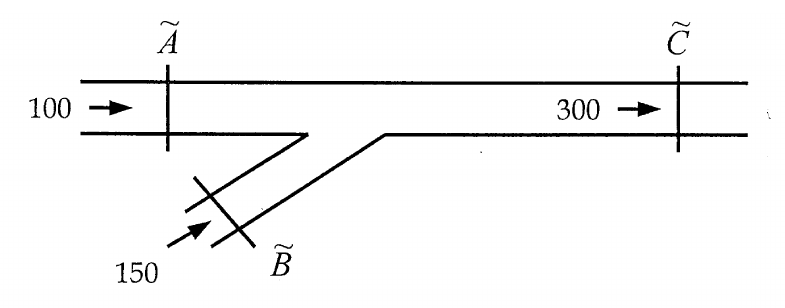
\includegraphics[width=0.5\textwidth]{traffic}
    \caption{نمونه مثال - ترافیک سنجیده شده در یک سه\ راهی}
    \label{fig:نمونه-مثال}
\end{figure}
فرض می\ کنیم که اعداد مشاهده شده، اعداد فازی هستند و به هریک مقادیر تابع عضویتی اختصاص می\ دهیم. بالاترین نقطه\ ی تابع عضویت می\ تواند معادل با مقدار مشاهده شده باشد. با توجه به دانشی که راجع به دقت مشاهدات صورت گرفته داریم، میزان پیشتیبانی\زیرنویس{\lr{Support}} هر تابع عضویت را مقداری فرض می\ کنیم.\بند
توابع عضویت مثلثی فرض می\ شوند ولی لزوما متقارن نیستند. اگر توابع عضویت برای هر مقدار را به صورت\ های
$h_A(x), h_B(y)$ و $h_C(z)$
فرض کنیم که
$A, B$ و $C$
مجموعه فازی از اعداد تقریبی فرض کنیم و همچنین
$x, y$ و $z$
اعداد نامعین\ ای که محدودیت تعریف شده را ارضا می\ کنند فرض کنیم؛ می\ توانیم مدل برنامه\ نویسی خطی ارائه شده زیر را را فرموله\ بندی کنیم:
\begin{latin}
\begin{table}[H]
    \begin{tabular}{ l l }
        Unknowns:       & $x$; $y$; $z$ and $h$\\
        Objective:      & Max $h$\\
        Constraints:    & The relationship, $x + y = z$\\
                        & $h \leq h_A(X)$, $h \leq h_B(X)$, $h \leq h_C(X)$,\\
                        & $x, y, z, h \geq 0$\\
    \end{tabular}  
\end{table}
\end{latin}
که در رابطه\ ی بالا $h$ کمترین درجه عضویت که یکی از مقادیر
$x, y$ و $z$
اختیار می\ کند می\ باشد، در فرموله\ بندی فوق همانطور که قبلا گفته شد به بدنبال مجموعه\ ای از مقادیر سازگار(قسمت \lr{Constraints}) هستیم که کوچکترین درجه عضویت($h^*$) بین آنها حداکثر شود(قسمت \lr{Objective}). به عبارت دیگر در برنامه\ نویسی خطی مقدار $h$ مشتق شده و $h^*$\؛ مقدار عضویت
$x, y$ و $z$
حداقل بزرگتر از $h^*$ می\ باشند:
\[h^* = Max\{Min[h_A(x), h_B(y), h_C(z)]\}\]
\begin{figure}[H]
    \centering
    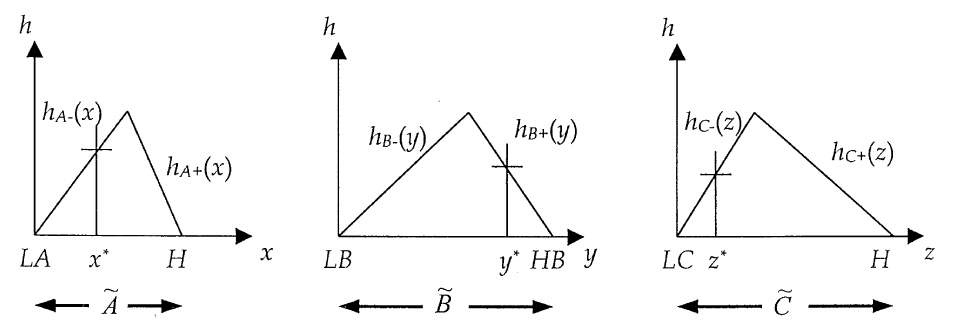
\includegraphics[width=0.75\textwidth]{prob-formul}
    \caption{فرموله\ سازی نمونه مثال شکل 
    \ref{fig:نمونه-مثال}}
    \label{fig:فرموله-سازی-نمونه-مثال}
\end{figure}
در شکل
\ref{fig:فرموله-سازی-نمونه-مثال}
اگر سمت چپ و راست توابع عضویت مثلثی را به ترتیب با نمادهای
$h_{\zeta_1-}(\zeta_2)$ و $h_{\zeta_1+}(\zeta_2)$
نمایش دهیم که
$(\zeta_1, \zeta_2) \in \{(A, x), (B, y), (C, z)\}$
می\ باشند و تابع مثلثی عضویت را به صورت
$\zeta_1 = (L\zeta_1, M\zeta_1, H\zeta_1)$
که به ترتیب (محدوده\ ی راست، مقدار میانی، محدوده\ ی چپ) پشتیبان هستند در نظر بگیریم؛ فرموله\ سازی پیشنهاد شده برای برنامه\ نویسی خطی فازی به صورت زیر است:
\begin{latin}
\begin{table}[H]
    \begin{tabular}{ l l }
        Maximize:       & $h$\\
        Subject to:     & $x + y = z$\\
                        & $h_{A-}(x) \geq h$, $h_{A+}(x) \geq h$\\
                        & $h_{B-}(x) \geq h$, $h_{B+}(x) \geq h$\\
                        & $h_{C-}(x) \geq h$, $h_{C+}(x) \geq h$\\
                        & $x, y, z, h \geq 0$\\
    \end{tabular}  
\end{table}
\end{latin}
که در بالا دو محدودیت سمت چپ و سمت راست تابع مثلثی عضویت برای هر یک از مشاهدات نیاز دارند که تعریف شوند.
\textbf{ایده\ ی کلی مقاله}
این است که با توجه به محدودیت\ های فرموله شده\ ی بالا بیاییم مقادیری غیرفازی برای هریک از مقادیر فازی مشاهده شده بیابیم و در طی این جستجو حداکثر سعی\ مان این باشد که این مقادیر غیرفازی به مقدار میانی مقادیر فازی مشاهده شده نزدیک باشند؛ و اینکه این جستجو مقدار را توسط برنامه\ نویسی خطی انجام می\ دهیم.\\
در مقاله با استفاده از مثال و بحث به توضیح روش و ایده ارائه شده پرداخته است که بعلت محدودیت صفحاتی انتسابی به تکلیف از توضیح بیشتر خودداری میکنم.
\vspace{10pt}\\
{\LARGE مرجع}
\renderref{reference}
\end{document}
